\chapter{Quantum Problems in Cosmology}
\label{chap:e23}

\begin{chapteropening}
In the previous chapters we pointed our telescopes at a star, an accretion disk, a burst: sources you can go back and look at again another night, whose bandwidth you can tune, whose experiment you can redo. The object of this chapter is one and only one, and it happens only once: \textbf{the entire universe}. It is an optical experiment that took place long ago and cannot be restarted; we merely set up our detector very late, to read a plate it left on the sky. This plate is the cosmic microwave background (cosmic microwave background, CMB): an almost perfect blackbody microwave sky, overlaid with temperature patterns of order \(10^{-5}\) and even fainter polarization structure.

This chapter answers three progressively deeper questions. First, \textbf{where do these patterns come from}? We will see that their seeds are the \emph{quantum} vacuum fluctuations amplified during inflation, together with one crucial turn: how these quantum fluctuations ``become,'' through decoherence, density perturbations describable by a classical random field. Second, \textbf{what does a beam of light experience crossing billions of light-years}? Its polarization may be quietly rotated by a small angle, and its arrival time may be pulled apart by the medium and by deeper physics. Third, \textbf{can we use a cosmologically long baseline to weigh the most fundamental physics}: Lorentz invariance, the upper limit on the photon mass? Bringing abstract cosmology, step by step, back down to the coherence, polarization, and photon arrival times familiar from this book.
\end{chapteropening}

\section{The universe as a one-shot optical experiment}
\label{sec:e23-lightfield}

Let us set the scene. When people talk about the CMB they open with ``inflationary quantum fluctuations,'' but the observational entry point is in fact very plain: the telescope first sees an almost perfect blackbody microwave sky, and then, on top of this mean background, measures a thin layer of angular fluctuations. So this section first weighs the CMB as a \emph{light field}, and then retreats all the way back to the early quantum modes that produced these patterns.

The mean CMB is a blackbody of temperature \(T_0=2.7255\pm0.0006\,{\rm K}\). Chapter~\ref{chap:e05} quantized the light field and wrote down the Planck blackbody formula, and Chapter~\ref{chap:e06} specifically discussed the thermal state (thermal state): in a thermal light field the mean photon occupation number of each frequency mode is given by the Bose distribution, and the specific intensity by the Planck formula:
\begin{equation}
  n_\nu=\frac{1}{\exp(h\nu/k_{\rm B}T_0)-1},
  \qquad
  I_\nu=\frac{2h\nu^3}{c^2}\,n_\nu .
  \label{eq:e23-planck-spectrum}
\end{equation}
\begin{formulaexplain}
\(n_\nu\) is the mean photon number in a single frequency mode, and \(I_\nu\) is the blackbody specific intensity. At the low-frequency end \(n_\nu\) is large and the field is close to classical thermal light; at the high-frequency end \(n_\nu<1\), and a single mode often has less than one photon.
\end{formulaexplain}
Symbol by symbol: \(\nu\) is in Hz, \(h\) is the Planck constant, \(k_{\rm B}\) is the Boltzmann constant, and \(I_\nu\) is in \({\rm erg\,s^{-1}\,cm^{-2}\,Hz^{-1}\,sr^{-1}}\) (the CMB literature often converts to \({\rm MJy\,sr^{-1}}\)). Plug in two real frequencies to get a feel: at \(30\,{\rm GHz}\), \(h\nu/k_{\rm B}T_0\simeq0.53\), so \(n_\nu\simeq1/(e^{0.53}-1)\simeq1.4\), and the low-frequency channel is still a near-classical thermal field; at \(150\,{\rm GHz}\), the exponent grows, \(n_\nu\simeq0.07\), and the single-mode occupation is already less than 1. The blackbody intensity peak falls near \(160\,{\rm GHz}\): this is precisely the physical reason the Planck high-frequency instrument and many ground experiments choose channels at \(90/150/220\,{\rm GHz}\). FIRAS measured this mean spectrum extremely close to an ideal blackbody, so modern cosmology simply treats the mean spectrum as a \emph{known background} and puts all the information into the angular fluctuations and polarization on top of it \citep{1994ApJ...420..439M,1996ApJ...473..576F,2009ApJ...707..916F}.

Expanding the fluctuations on the sky into spherical harmonics (spherical harmonics) is like expanding a stretch of sound into different pitches:
\begin{equation}
  T(\hat{\bm n})=T_0\,[1+\Theta(\hat{\bm n})],
  \qquad
  \Theta(\hat{\bm n})=\sum_{\ell m}a^{T}_{\ell m}\,Y_{\ell m}(\hat{\bm n}).
  \label{eq:e23-temperature-expansion}
\end{equation}
\begin{formulaexplain}
\(\Theta\) is the dimensionless temperature fluctuation, \(a^{T}_{\ell m}\) are the spherical-harmonic coefficients, and \(Y_{\ell m}\) are the spherical-harmonic functions. This expression breaks a sky map into layers of angular scale: \(\ell\) sets the scale, and \(m\) governs the azimuthal pattern at the same scale.
\end{formulaexplain}
Here \(\hat{\bm n}\) is the sky direction (a unit vector), and the multipole \(\ell\) is approximately related to angular scale by \(\theta\simeq180^\circ/\ell\): \(\ell\simeq2\) is a pattern as large as half the sky, \(\ell\simeq200\) is about one degree, and \(\ell\simeq2000\) is only a few arcminutes. The differential microwave radiometer of COBE first saw \(\Delta T/T\sim10^{-5}\) structure on an all-sky map, and Planck decomposed it all the way to \(\ell\sim2500\). For an isotropic Gaussian sky, squaring and averaging all the \(m\) at the same \(\ell\) gives the angular power spectrum (angular power spectrum):
\begin{equation}
  \widehat C^{TT}_\ell=\frac{1}{2\ell+1}\sum_{m=-\ell}^{\ell}\bigl|a^{T}_{\ell m}\bigr|^2,
  \qquad
  D^{TT}_\ell=\frac{\ell(\ell+1)}{2\pi}\,C^{TT}_\ell .
  \label{eq:e23-cl-estimator}
\end{equation}
\begin{formulaexplain}
\(\widehat C^{TT}_\ell\) is the temperature angular-power-spectrum estimator, from the average of all \(2\ell+1\) modes \(m\) at one \(\ell\); \(D_\ell\) is the rescaled form commonly used for plotting. This average is the core compression of the CMB two-point statistics.
\end{formulaexplain}
If \(a_{\ell m}\) is in units of \(\mu{\rm K}\), then \(C_\ell\) and \(D_\ell\) are in \(\mu{\rm K}^2\). The first acoustic peak of \(D^{TT}_\ell\) is at \(\ell\simeq220\), with a peak height of about \(5\times10^3\,\mu{\rm K}^2\). These peaks are not random; they come from the \emph{acoustic oscillations} of the photon--baryon fluid before recombination (recombination): the baryon density changes the height of the compression peaks, the dark-matter density changes the decay of the gravitational potential, and the angular diameter distance projects the physical acoustic scale onto an angular scale on the sky. Planck fits these peaks with a six-parameter flat \(\Lambda{\rm CDM}\) model, giving typical precision such as \(\Omega_bh^2\simeq0.0224\), \(\Omega_ch^2\simeq0.120\), \(n_s\simeq0.965\), \(H_0\simeq67.4\,{\rm km\,s^{-1}\,Mpc^{-1}}\) \citep{1992ApJ...396L...1S,1996ApJ...469..437S,2020A&A...641A...5P,2020A&A...641A...6P}. Here \(\Omega_x\) is the dimensionless density parameter of the \(x\)-th component (the ratio of that component's density to the critical density), \(h\equiv H_0/(100\,{\rm km\,s^{-1}\,Mpc^{-1}})\) is the reduced Hubble constant, and the reason for writing the combination \(\Omega h^2\) is that what the CMB directly constrains is the physical density, independent of the value of \(H_0\): these are all outputs of the six-parameter fit, and if one wishes to examine the origin of the notation in detail, consult any cosmology textbook; this book merely uses them as known numbers.

Here is a ``happens only once'' cosmology-specific limitation. Even if the instrument were perfect and noiseless, at each \(\ell\) the sky gives you only \(2\ell+1\) modes \(m\), that is all the sample there is, and the variance cannot be dodged. This is called cosmic variance (cosmic variance):
\begin{equation}
  \frac{\sigma(C_\ell)}{C_\ell}=\sqrt{\frac{2}{(2\ell+1)\,f_{\rm sky}}} .
  \label{eq:e23-cosmic-variance}
\end{equation}
\begin{formulaexplain}
\(\sigma(C_\ell)/C_\ell\) is the relative error from sample variance, and \(f_{\rm sky}\) is the effective sky fraction. Low \(\ell\) has few usable modes, so large angular scales inherently carry a layer of statistical uncertainty that cannot be removed by sensitivity.
\end{formulaexplain}
\(f_{\rm sky}\) is the fraction of the sky used (the Galactic plane and strong foregrounds must be masked, so usually \(f_{\rm sky}<1\)). Plug in numbers: the relative error at all-sky \(\ell=2\) is about \(\sqrt{2/5}\simeq63\%\), dropping to about \(7\%\) at \(\ell=200\), and only about \(2.2\%\) at \(\ell=2000\). This is why phenomena such as ``low-\(\ell\) anomalies'' and ``a low quadrupole'' must be judged within the covariance of a finite number of modes, and not merely because they look conspicuous on the plot. This is of one spirit with the error budget of Chapter~\ref{chap:e15}: first ask ``how much independent information do I actually have.''

The polarization map has two more Stokes parameters, \(Q\) and \(U\), than the temperature map. They are not scalars, but \emph{spin-2} (spin-2) quantities that rotate with the coordinates, so they must be expanded in spin-weighted spherical harmonics and then linearly combined into two modes of definite parity:
\begin{equation}
  (Q\pm iU)(\hat{\bm n})=\sum_{\ell m}a_{\pm2,\ell m}\,{}_{\pm2}Y_{\ell m}(\hat{\bm n}),
  \quad
  a^{E}_{\ell m}=-\tfrac12(a_{2,\ell m}+a_{-2,\ell m}),
  \quad
  a^{B}_{\ell m}=\tfrac{i}{2}(a_{2,\ell m}-a_{-2,\ell m}).
  \label{eq:e23-eb-definition}
\end{equation}
\begin{formulaexplain}
\(Q\pm iU\) are the spin-\(\pm2\) polarization fields, \({}_{\pm2}Y_{\ell m}\) are the spin-weighted spherical harmonics, and \(a^{E/B}_{\ell m}\) are the E/B-mode coefficients. This combination translates the pointwise polarization direction into two classes of all-sky patterns.
\end{formulaexplain}
The key physics lies in parity: the \(E\) mode behaves like a scalar under a mirror transformation (the polarization directions form a radial or concentric pattern around hot and cold spots), while the \(B\) mode behaves like a pseudoscalar (with a vortical feel). Linear-order scalar density fluctuations produce mainly \(T\) and \(E\), and do \emph{not} directly produce primordial \(B\). Only a few things can produce \(B\): primordial tensor perturbations (gravitational waves), weak gravitational lensing, an overall rotation of the polarization angle, and Galactic dust and synchrotron foregrounds. Keep this in mind: \textbf{\(B\) modes are rare guests}, and whoever can cleanly create them carries the deepest cosmological information. This thread will be pulled twice later in this chapter: once toward primordial gravitational waves, once toward polarization birefringence. These two light-field skeleton diagrams are shown in Figures~\ref{fig:e23-blackbody} and \ref{fig:e23-power}.

\begin{figure}[tbp]
\centering
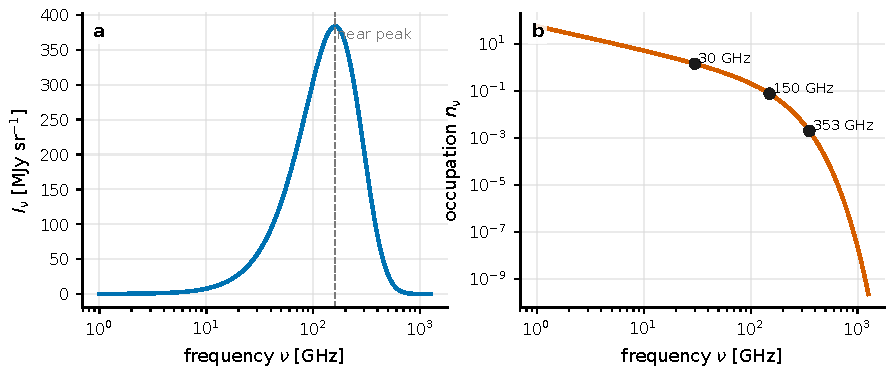
\includegraphics[width=0.9\linewidth]{figures/generated/chapter_16/ch16_cmb_blackbody.pdf}
\caption{The mean light field of the CMB is determined jointly by the blackbody spectrum and the mode occupation number. The left panel writes the Planck spectrum at \(T_0=2.7255\,{\rm K}\) in \({\rm MJy\,sr^{-1}}\), peaking near \(160\,{\rm GHz}\); the right panel is the single-mode mean photon number \(n_\nu\) of the same blackbody at different frequencies, with the low-frequency channels having higher occupation and the high-frequency channels gradually entering \(n_\nu<1\).}
\label{fig:e23-blackbody}
\end{figure}

\begin{figure}[tbp]
\centering
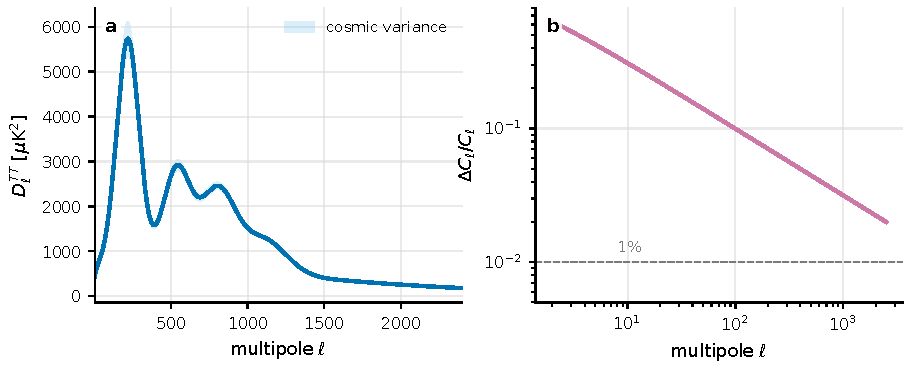
\includegraphics[width=0.9\linewidth]{figures/generated/chapter_16/ch16_cmb_power_spectrum.pdf}
\caption{The angular power spectrum compresses the sky fluctuations into multipole space. The left panel is \(D_\ell^{TT}\) with acoustic peaks and a damping tail, with the shading showing the order of magnitude of all-sky cosmic variance; the right panel plots \(\sqrt{2/(2\ell+1)}\) alone, showing that the error at large angular scales is set by the number of usable modes on the sky, a variance no amount of telescope sensitivity can remove.}
\label{fig:e23-power}
\end{figure}

\section{Inflation: amplifying vacuum fluctuations into density perturbations}
\label{sec:e23-inflation}

The \(C_\ell\) of the previous section is a statistic on the sky; what inflation (inflation) theory must explain is why these statistics are \emph{nearly Gaussian}, \emph{nearly scale-invariant}, and why the phases of the acoustic peaks are fixed (not a jumble of random-phase noise). Here we cannot treat the CMB as a laboratory beam that can be repeatedly prepared, but must regard every field mode in the early universe as the familiar quantum harmonic oscillator of Chapter~\ref{chap:e04}, only its frequency varies with cosmic expansion.

For the scalar curvature perturbation \(\mathcal R\), one defines a Mukhanov--Sasaki variable \(v\) that ``packages'' the background evolution in:
\begin{equation}
  v(\bm x,\eta)=z(\eta)\,\mathcal R(\bm x,\eta),
  \qquad
  z=\frac{a\,\dot\phi}{H} .
  \label{eq:e23-ms-variable}
\end{equation}
\begin{formulaexplain}
\(v\) is the Mukhanov--Sasaki variable, \(\mathcal R\) is the curvature perturbation we ultimately care about, and \(z=a\dot\phi/H\) packs the background evolution of inflation into a single coefficient. Writing the equations with \(v\), each Fourier mode becomes a quantum harmonic oscillator with a time-varying frequency.
\end{formulaexplain}
Symbol by symbol: \(\eta\) is conformal time (conformal time, satisfying \({\rm d}\eta={\rm d}t/a\)), \(a\) is the scale factor (dimensionless, set to 1 today), \(\phi\) is the background scalar field driving inflation, \(H=\dot a/a\) is the Hubble rate (in \({\rm s^{-1}}\)), and the dot denotes a derivative with respect to cosmic time. Expanding the second-order action for each Fourier mode \(v_k\) yields an equation of motion of extremely clean form:
\begin{equation}
  v_k''+\Bigl(k^2-\frac{z''}{z}\Bigr)v_k=0 .
  \label{eq:e23-ms-equation}
\end{equation}
\begin{formulaexplain}
\(v_k\) is the mode function of comoving wavenumber \(k\), and the prime is a derivative with respect to conformal time \(\eta\). The \(k^2-z''/z\) in the brackets is the squared effective frequency of this ``time-varying oscillator,'' and the flip of its sign is precisely all the magic of inflation.
\end{formulaexplain}
\(k\) is the comoving wavenumber (comoving wavenumber, in \({\rm Mpc^{-1}}\)). The two limits of this equation determine everything; let us read them out one by one:

\emph{Sub-horizon} (\(k\gg aH\)): \(z''/z\) is negligible compared with \(k^2\), and the equation degenerates into \(v_k''+k^2v_k=0\), an ordinary simple harmonic oscillator. Taking its quantum vacuum (the Bunch--Davies vacuum), the normalized mode function is
\[
  v_k(\eta)\simeq\frac{e^{-ik\eta}}{\sqrt{2k}} .
\]
This is precisely the vacuum fluctuation of ``the lowest energy state still jittering'' that this book has discussed from the very beginning, only occurring on every short-wave mode of the early universe.

\emph{Horizon exit} (\(k\simeq aH\), and thereafter \(k\ll aH\)): expansion pushes \(z''/z\) up so that it dominates the equation. Now the growing solution no longer oscillates but is \emph{frozen}, the decaying solution shrinks rapidly, and \(\mathcal R_k=v_k/z\) tends to a nearly constant. ``Frozen'' does not mean the mode stops evolving, but that one direction in phase space is strongly narrowed, leaving in the end only a single random amplitude to govern the later density perturbations \citep{1988JETP...67.1297M,1990PhRvD..42.3413G,1996CQGra..13..377P}.

Writing this frozen two-point statistic as the dimensionless primordial curvature power spectrum:
\begin{equation}
  \langle\mathcal R_{\bm k}\mathcal R_{\bm k'}\rangle
  =(2\pi)^3\delta^{(3)}(\bm k+\bm k')\,\frac{2\pi^2}{k^3}\,\mathcal P_{\mathcal R}(k),
  \qquad
  \mathcal P_{\mathcal R}(k)=A_s\Bigl(\frac{k}{k_*}\Bigr)^{n_s-1} .
  \label{eq:e23-primordial-spectrum}
\end{equation}
\begin{formulaexplain}
\(\mathcal P_{\mathcal R}\) is the dimensionless primordial curvature power spectrum, \(A_s\) is the amplitude, \(n_s\) is the spectral index (spectral index), and \(k_*\) is the reference wavenumber (pivot). It condenses the early quantum fluctuations' two-point statistics into the two most central numbers of today's CMB fits.
\end{formulaexplain}
Planck commonly takes the pivot \(k_*=0.05\,{\rm Mpc^{-1}}\), giving \(\ln(10^{10}A_s)\simeq3.04\), i.e.\ \(A_s\simeq2.1\times10^{-9}\). The spectral index \(n_s=1\) is exact scale invariance; the measured \(n_s\simeq0.965\) shows a slight ``red tilt,'' the long waves slightly stronger than the short waves, precisely the small deviation expected from slow-roll inflation. Keep this order-of-magnitude chain firmly in mind: a primordial curvature power of \(10^{-9}\), passed through the radiation transfer function, the acoustic oscillations, the finite thickness of the recombination surface, and later lensing smoothing, is projected into the patterns of \(\Delta T/T\sim10^{-5}\) on the sky today \citep{2020A&A...641A...6P,2020A&A...641A..10P}.

Now let us translate it into the quantum-optics language of this book. The time-varying background of inflation evolves the pair of modes \(\bm k\) and \(-\bm k\) from the vacuum into a \emph{two-mode squeezed state} (two-mode squeezed state), as was said when introducing squeezed states in Chapter~\ref{chap:e06}, squeezing means ``amplifying the fluctuations of a pair of modes in pairs, while maintaining a fixed phase relation'':
\begin{equation}
  |\psi\rangle=\prod_{\bm k}\exp\!\Bigl[\,r_k e^{-2i\varphi_k}\,\hat a_{\bm k}\hat a_{-\bm k}
  -r_k e^{2i\varphi_k}\,\hat a^\dagger_{\bm k}\hat a^\dagger_{-\bm k}\Bigr]\,|0\rangle .
  \label{eq:e23-squeezed-state}
\end{equation}
\begin{formulaexplain}
\(|\psi\rangle\) is the two-mode squeezed state of the pair \(\bm k\) and \(-\bm k\), \(r_k\) is the squeezing strength, \(\varphi_k\) is the squeezing angle, and \(\hat a,\hat a^\dagger\) are the annihilation and creation operators. Inflation amplifies the vacuum fluctuations in pairs and locks their phases.
\end{formulaexplain}
The mean occupation number of each pair of modes is \(N_k=\sinh^2 r_k\). After \(50\text{--}60\) e-folds (the logarithm of the amount of expansion), \(r_k\) is very large, and \(N_k\) grows exponentially. A reminder: the ``occupation number'' here refers to the number of quantum excitations of the early \emph{field modes}, which is not the same thing as the number of CMB photons the telescope actually counts today. In phase space, squeezing stretches the Wigner function into a very thin, elongated ellipse: one direction is stretched long (the one that later serves as the classical random amplitude), and the other is squeezed very narrow. It is precisely this squeezed-dead direction that locks the fixed phase, thereby arranging a regular string of acoustic peaks in the \(TT\), \(TE\), \(EE\) spectra, rather than random noise (Figure~\ref{fig:e23-squeezed}) \citep{1990PhRvD..42.3413G,1996CQGra..13..377P,2006CQGra..23.2317P}.

\begin{figure}[tbp]
\centering
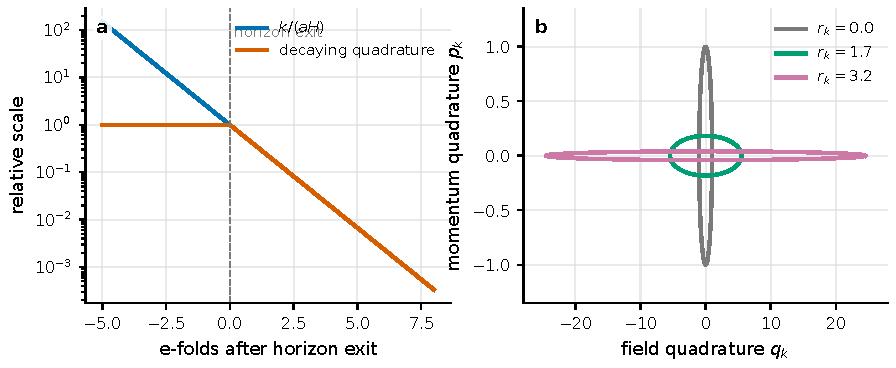
\includegraphics[width=0.9\linewidth]{figures/generated/chapter_16/ch16_squeezed_modes.pdf}
\caption{Mode amplification during inflation can be viewed as two-mode squeezing. The left panel shows \(k/(aH)\) falling exponentially after horizon exit, with the decaying direction squeezed narrow; the right panel plots the phase-space ellipse, with one direction stretched long and the other squeezed dead as \(r_k\) grows, and what is observed is the long axis, which later behaves as the classical random amplitude.}
\label{fig:e23-squeezed}
\end{figure}

\section{Decoherence: how quantum fluctuations ``become'' classical density perturbations}
\label{sec:e23-decoherence}

The previous section left an unease: if each mode is still a pure quantum squeezed state, it is a quantum superposition: how can it be used directly as a classical density fluctuation to compute how galaxies grow? The answer is decoherence (decoherence). This is also the first true ``quantum problem'' of this chapter: \textbf{why does an amplified quantum state behave observationally like a classical random field}?

First a picture. The ``quantumness'' of a quantum state is hidden in the \emph{off-diagonal terms} of its density matrix: the evidence that different amplitude branches can still interfere with each other. But these inflationary modes are not isolated: they are entangled with a great mass of unobserved degrees of freedom (unobserved short-wave modes, tensor--scalar interactions, degrees of freedom of the pre-recombination plasma, the lensing potential, and even the foreground and instrument modes marginalized away in data analysis). Once these environments are summed and integrated out, the off-diagonal terms of the reduced density matrix of the observed variable \(q_k\) are rapidly flattened by a Gaussian factor:
\begin{equation}
  \rho_{\rm red}(q,q')=\rho_0(q,q')\,\exp\!\bigl[-\Gamma_k\,(q-q')^2\bigr] .
  \label{eq:e23-decoherence-density}
\end{equation}
\begin{formulaexplain}
\(\rho_{\rm red}\) is the reduced density matrix of the observed variable \(q_k\), \(\rho_0\) is the undecohered form, and \(\Gamma_k\) measures the strength with which the environment flattens the off-diagonal terms. When the coherence term for \(q\ne q'\) is squeezed dead, the power spectrum can be computed with a classical random field.
\end{formulaexplain}
Reading this expression word by word: \(q,q'\) are two different values of the same observed variable, and a larger \((q-q')\) means the two branches are farther apart; the exponential factor \(\exp[-\Gamma_k(q-q')^2]\) is a bell-shaped ``valve'' that almost completely shuts off the interference between branches that are farther apart. The dimension of \(\Gamma_k\) depends on how \(q_k\) is normalized, but the physical criterion is crisp: as long as \(\Gamma_k(\Delta q)^2\gg1\), the different amplitude branches will never again interfere, and the two-point function, the angular power spectrum \(C_\ell\), the angular bispectrum (bispectrum), and lensing reconstruction can all be computed honestly with a classical random field. For inflationary modes, the stronger the squeezing and the deeper the entanglement, the larger \(\Gamma_k\), and this condition is enormously satisfied. This is precisely the exact meaning of the sentence ``quantum fluctuations become classical density perturbations.''

To prevent misunderstanding, a word about the boundary. Decoherence makes the \emph{statistics} classical, but it does not answer for us ``which branch was actually realized'': the ``measurement problem'' of the early universe remains conceptually debated. However, for the quantities we can measure (\(C_\ell\), lensing reconstruction, higher-order correlations), the residual coherent phase information is too little, long since insufficient to support a laboratory-style Bell test, and unable to treat the CMB as a repeatedly preparable non-classical state to manipulate \citep{1996CQGra..13..377P,2006CQGra..23.2317P}. This stands in contrast with the quantum-network telescope of Chapter~\ref{chap:e24}: there you can actively prepare, modulate, and re-measure a quantum state; here, the universe gives you only a plate that cannot be re-shot, and the quantumness ``settled'' into classical statistics long before recombination.

\section{How the fluctuations are produced: non-Gaussianity and primordial gravitational waves}
\label{sec:e23-tensors}

The two-point function (that is, \(C_\ell\)) tells us \emph{how much} fluctuation there is; to ask \emph{how} these fluctuations were produced, one must look at two harder-to-measure things: higher-point functions (non-Gaussianity) and tensor modes (primordial gravitational waves). The former tests the interactions and field content during inflation, the latter points directly at whether a primordial gravitational-wave background exists. Both are extremely tempting, and both are extremely easily limited by the finite number of modes, lensing, dust, and template choice.

If \(\mathcal R\) is a strictly Gaussian field, all the information is in the two-point function, and the three-point and above are all zero. But as soon as inflation has interactions, a non-trivial sound speed, multi-field transfer, or a sharp feature, non-Gaussianity leaks out. Its protagonist is the three-point function:
\begin{equation}
  \langle\mathcal R_{\bm k_1}\mathcal R_{\bm k_2}\mathcal R_{\bm k_3}\rangle
  =(2\pi)^3\delta^{(3)}(\bm k_1+\bm k_2+\bm k_3)\,B_{\mathcal R}(k_1,k_2,k_3) .
  \label{eq:e23-bispectrum}
\end{equation}
\begin{formulaexplain}
\(B_{\mathcal R}\) is the three-point spectrum (bispectrum) of the curvature perturbation, and the delta function forces the three wavevectors to join head to tail and close into a triangle. The \emph{shape} of the triangle corresponds to different early-universe interactions, so the three-point function is the main language of non-Gaussianity.
\end{formulaexplain}
Different ``shapes'' give different signals: the local type is strongest in \emph{squeezed} triangles (\(k_1\ll k_2\simeq k_3\)), the equilateral type is strongest in \emph{equilateral} triangles, and the orthogonal type is an approximately orthogonal template artificially constructed to distinguish different interactions. The local type has a very intuitive real-space writing:
\begin{equation}
  \mathcal R(\bm x)=\mathcal R_g(\bm x)+\frac{3}{5}f^{\rm local}_{\rm NL}
  \Bigl[\mathcal R_g^2(\bm x)-\langle\mathcal R_g^2\rangle\Bigr] .
  \label{eq:e23-local-fnl}
\end{equation}
\begin{formulaexplain}
\(\mathcal R_g\) is a pure Gaussian field, and \(f^{\rm local}_{\rm NL}\) is the amplitude of the local-type non-Gaussianity. That quadratic term lets \emph{long waves} modulate the power of \emph{short waves}, so the local template is most sensitive in squeezed triangles.
\end{formulaexplain}
\(f_{\rm NL}\) is dimensionless. Planck, using temperature plus polarization, gives \(f^{\rm local}_{\rm NL}=-0.9\pm5.1\), \(f^{\rm equil}_{\rm NL}=-26\pm47\), \(f^{\rm orth}_{\rm NL}=-38\pm24\) (\(68\%\) confidence), all consistent with zero: no significant non-Gaussianity found under the standard templates (Figure~\ref{fig:e23-nongaussian}). This is in fact strong support for the simplest inflation: single-field slow-roll inflation has a ``consistency relation'' predicting minimal local non-Gaussianity in the squeezed limit, of order comparable to \(1-n_s\) (i.e.\ a few percent), so \(f_{\rm NL}\) should naturally be very small \citep{2003JHEP...05..013M,2020A&A...641A...9P,2020A&A...641A..10P}.

\begin{figure}[tbp]
\centering
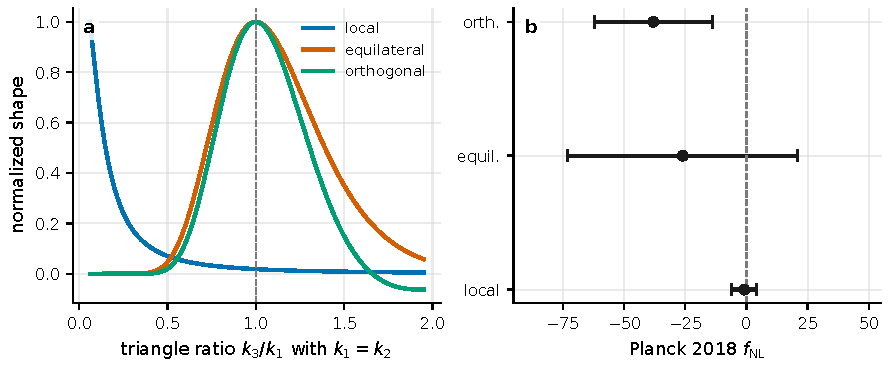
\includegraphics[width=0.9\linewidth]{figures/generated/chapter_16/ch16_non_gaussian_templates.pdf}
\caption{Non-Gaussianity is determined jointly by the triangle configuration and the amplitude. The left panel uses a \(k_1=k_2\) slice to compare the shapes of the local, equilateral, and orthogonal templates; the local type is enhanced in the squeezed limit, and the equilateral type is maximal when the three sides are nearly equal. The right panel gives Planck's representative constraints on the three commonly used \(f_{\rm NL}\), with all error bars consistent with zero.}
\label{fig:e23-nongaussian}
\end{figure}

Tensor perturbations are the most direct CMB target of a quantum-gravity background: they are the primordial gravitational waves produced by inflation, and will leave that ``rare guest,'' the \(B\) mode, in the polarization. People measure them with the ratio of tensor to scalar power:
\begin{equation}
  r(k_*)=\frac{\mathcal P_t(k_*)}{\mathcal P_{\mathcal R}(k_*)},
  \qquad
  \mathcal P_t(k)=A_t\Bigl(\frac{k}{k_*}\Bigr)^{n_t} .
  \label{eq:e23-tensor-r}
\end{equation}
\begin{formulaexplain}
\(r\) is the ratio of the tensor power spectrum to the scalar curvature power spectrum at the pivot \(k_*\), and \(\mathcal P_t\) is described by the amplitude \(A_t\) and the tensor tilt \(n_t\). It compresses the primordial gravitational-wave background into a single number most often cited in CMB \(B\)-mode searches.
\end{formulaexplain}
\(r\) is dimensionless, but the pivot is commonly taken as \(0.002\) or \(0.05\,{\rm Mpc^{-1}}\), and the two \emph{cannot be mixed}. Single-field slow-roll gives another consistency relation \(n_t\simeq-r/8\). \(r\) is precious because it directly converts into the energy scale at which inflation occurred:
\begin{equation}
  V_*^{1/4}\simeq1.06\times10^{16}\,{\rm GeV}\Bigl(\frac{r}{0.01}\Bigr)^{1/4} .
  \label{eq:e23-inflation-scale}
\end{equation}
\begin{formulaexplain}
\(V_*^{1/4}\) is the energy scale of inflation, and \(r\) is the tensor-to-scalar ratio. Note that \emph{fourth root}: even if the upper limit on \(r\) improves by a large margin, the energy-scale constraint tightens only slowly.
\end{formulaexplain}
This expression assumes Einstein gravity, standard slow-roll, and a single energy scale. Planck alone gives \(r_{0.002}<0.10\) (\(95\%\) confidence); combined with the \(B\)-mode polarization of BICEP/Keck it tightens to \(r_{0.002}<0.056\), corresponding to \(V_*^{1/4}<1.6\times10^{16}\,{\rm GeV}\), already approaching the grand-unification scale. BICEP/Keck, combining the 2018-season data with Planck and WMAP, further gives \(r_{0.05}<0.036\), and points out that the current limit is bottlenecked simultaneously by lensing \(B\) modes and Galactic dust (Figure~\ref{fig:e23-bmode}) \citep{2020A&A...641A..10P,2021PhRvL.127o1301A,2019JCAP...02..056A}. In other words, the difficulty of catching that ``rare guest'' lies not in sensitivity but in first ushering out, one by one, the lensing and dust that impersonate it.

\begin{figure}[tbp]
\centering
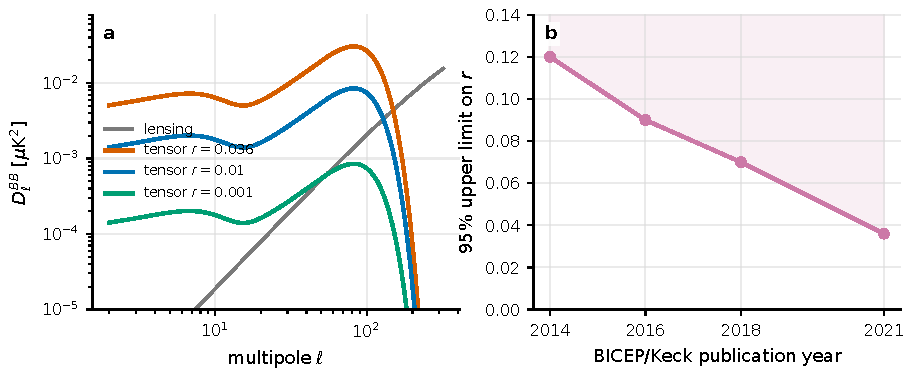
\includegraphics[width=0.9\linewidth]{figures/generated/chapter_16/ch16_bmode_constraints.pdf}
\caption{Tensor modes are constrained mainly through \(B\)-mode polarization. The left panel compares the lensing \(B\) mode with the primordial tensor \(B\) mode for different \(r\): the recombination peak at \(\ell\sim80\) is the main battlefield of ground experiments, while the low-\(\ell\) reionization peak requires large sky areas. The right panel shows the joint constraints of the BICEP/Keck series improving all the way from \(r<0.12\) to the order of \(r_{0.05}<0.036\).}
\label{fig:e23-bmode}
\end{figure}

\section{Photons crossing the universe: polarization is quietly rotated by an angle}
\label{sec:e23-birefringence}

The previous sections were all about ``how the plate was exposed.'' Now switch perspective: light sets out from the last-scattering surface and travels nearly the whole age of the universe to reach us: \textbf{will it be rewritten along the way}? The first precisely testable effect is polarization birefringence (cosmic birefringence): if there exists an extremely light, axion-like (axion) field coupled to the electromagnetic field, the linear-polarization direction of light will be rotated as a whole by a small angle \(\beta\) during propagation. Chapter~\ref{chap:e22} wrote about this polarization channel from the angle of dark matter and axions; here we look at what troubles it meets when it lands on the CMB.

The trouble is first a \emph{calibration} problem. Rotating the polarization direction of the whole sky by \(\beta\) leaks part of the \(E\) mode into the \(B\) mode, producing a signal in the \(EB\) and \(TB\) cross-spectra that should be zero. At small angles this leakage is approximately
\[
  \frac{C_\ell^{EB}}{C_\ell^{EE}-C_\ell^{BB}}\simeq \tfrac12\tan 4\beta\simeq 2\beta .
\]
Plug in a number to feel the order of magnitude: \(0.35^\circ=6.1\times10^{-3}\,{\rm rad}\), so \(2\beta\simeq1.2\%\). This one-percent signal falls precisely at an awkward position: large enough to leave a statistical trace in Planck-level all-sky data, and small enough that \emph{any} inaccuracy in the absolute polarization-angle calibration, dust's own \(EB\), bandpass mismatch, or beam leakage can impersonate it. The lethal part is that a true cosmic rotation angle \(\beta\) and an overall detector polarization-angle miscalibration \(\alpha\) act in almost the same direction in \(EB/TB\), so using only the CMB, what you measure is in fact \(\alpha+\beta\). The key to separating the two is frequency: the cosmological rotation treats all frequencies alike, while the Galactic foreground's polarization varies with frequency, and detector miscalibration is a per-frequency instrumental quantity.

Minami and Komatsu used precisely this ``frequency key,'' relying on the Galactic foreground's different behavior at different frequencies to estimate simultaneously the per-frequency instrumental miscalibration \(\alpha_\nu\) and the cosmic rotation \(\beta\), obtaining \(\beta=0.35\pm0.14^\circ\), and stripping the ground-based angle-calibration systematic of about \(0.28^\circ\) out of the final error. A subsequent analysis using WMAP+Planck PR4, adding a dust \(EB\) model over \(23\text{--}353\,{\rm GHz}\), gives a near-all-sky \(\beta=0.342^{+0.094}_{-0.091}{}^\circ\), with a significance of about \(3.6\sigma\), but polarized dust's own \(EB\), low-frequency synchrotron \(EB\), and independent angle calibration remain the main limitations (Figure~\ref{fig:e23-biref}) \citep{2020PhRvL.125v1301M,2022PhRvD.106f3503E,2022PhRvL.128i1302D,2022NatRP...4..452K}. If interpreted as an axion-like field, the rotation angle comes from the difference of the field value at the two ends of propagation:
\begin{equation}
  \beta=\frac12\,g_{\phi\gamma}\,\bigl[\phi(t_0)-\phi(t_{\rm LSS})\bigr] .
  \label{eq:e23-axion-birefringence}
\end{equation}
\begin{formulaexplain}
\(\beta\) is the global rotation angle of the CMB polarization, \(g_{\phi\gamma}\) is the coupling constant of the field to photons, and the brackets are the difference of the field value between today \(t_0\) and the last-scattering surface \(t_{\rm LSS}\). If the rotation truly comes from an axion-like propagation effect, it should be \emph{approximately frequency-independent}.
\end{formulaexplain}
\(g_{\phi\gamma}\) is in \({\rm GeV^{-1}}\), and \(\phi\) is the effective field value from the last-scattering surface to today. This expression assumes the rotation is approximately isotropic, frequency-independent, and originates from \emph{propagation} rather than an intrinsic \(EB\) at the emission surface. Conversely, the frequency dependence is the best diagnostic: if \(\beta(\nu)\propto\nu^{-2}\), it is more like Faraday rotation through a magnetized plasma (the propagation effect of Chapter~\ref{chap:e21}) than an axion; if \(\beta\) varies with sky region, redshift, or time, then a global angle must be generalized to a direction-dependent or time-dependent correlation function. The pedagogical point here is worth remembering: \textbf{in cosmology, a ``signal'' and a ``calibration error'' often look exactly alike, and separating them relies frequently not on a more sensitive detector, but on cleverer use of extra dimensions like frequency and sky region.}

\begin{figure}[tbp]
\centering
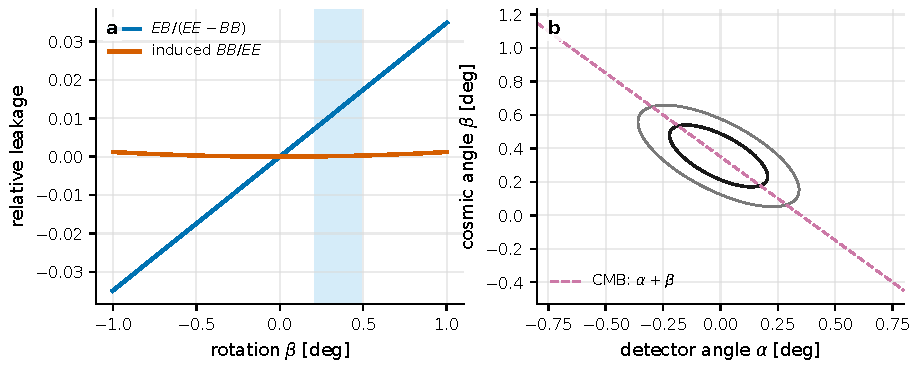
\includegraphics[width=0.9\linewidth]{figures/generated/chapter_16/ch16_birefringence_eb.pdf}
\caption{CMB birefringence puts the polarization-angle error and the cosmological signal on the same plane. The left panel shows the small-angle leakage of \(\beta\) into \(EB\) and induced \(BB\), with the shading marking the order of magnitude of \(\beta=0.35\pm0.14^\circ\); the right panel shows the degeneracy direction of the detector angle \(\alpha\) and the cosmic angle \(\beta\): using only the CMB one measures mainly \(\alpha+\beta\), and only adding foreground frequency information can possibly separate the two.}
\label{fig:e23-biref}
\end{figure}

\section{Arrival time and dispersion: weighing fundamental physics with a cosmological baseline}
\label{sec:e23-timing}

Polarization rotated by an angle is one way light is rewritten en route; \textbf{arrival time pulled apart} is another. This section moves the two tools this book values most, the high-time-resolution photon event table (Chapter~\ref{chap:e13}) and transient sources (the fast radio bursts, gamma-ray bursts, and pulsars of Chapter~\ref{chap:e20}), together onto a cosmological baseline, to test the most fundamental physics: is the speed of light really independent of frequency? Is the photon really strictly massless? Does Lorentz invariance still hold at extremely high energies?

The core of the idea is a criterion plainer than anything: \textbf{if a burst emitted light of various frequencies in the same instant, and they did not arrive simultaneously, then ``something happened along the way''}. To turn this sentence into a measurable, one must write down the relation between frequency and propagation speed. First look at the most familiar, and the first to be subtracted: the tenuous interstellar and intergalactic plasma. The dispersion relation (dispersion relation) an electromagnetic wave satisfies in cold plasma is
\begin{equation}
  \omega^2=\omega_p^2+c^2k^2,
  \qquad
  \omega_p^2=\frac{4\pi n_e e^2}{m_e}.
  \label{eq:e23-plasma-dispersion}
\end{equation}
\begin{formulaexplain}
\(\omega\) is the angular frequency, \(k\) is the wavenumber, \(\omega_p\) is the plasma frequency, \(n_e\) is the electron number density, and \(e,m_e\) are the electron charge and mass (CGS system). The plasma adds a \emph{constant term} \(\omega_p^2\) to the dispersion relation, and the wave can propagate only when \(\omega>\omega_p\).
\end{formulaexplain}
The group velocity (the speed the signal actually travels) is \(v_g={\rm d}\omega/{\rm d}k\). Solving \(k=\sqrt{\omega^2-\omega_p^2}/c\) from \eqref{eq:e23-plasma-dispersion}, differentiating both sides with respect to \(\omega\) and taking the reciprocal, with no skipped step:
\[
  \frac{{\rm d}k}{{\rm d}\omega}=\frac{1}{c}\frac{\omega}{\sqrt{\omega^2-\omega_p^2}}
  \;\Longrightarrow\;
  v_g=\frac{{\rm d}\omega}{{\rm d}k}=c\,\frac{\sqrt{\omega^2-\omega_p^2}}{\omega}
  =c\sqrt{1-\frac{\omega_p^2}{\omega^2}}
  \simeq c\Bigl(1-\frac{\omega_p^2}{2\omega^2}\Bigr),
\]
where the last step used the Taylor expansion \(\sqrt{1-x}\simeq1-x/2\) for \(\omega_p\ll\omega\). The time to travel a path length \(L\) is \(t=L/v_g\simeq(L/c)(1+\omega_p^2/2\omega^2)\). So for two frequencies \(\omega_1<\omega_2\) emitted simultaneously, the difference in arrival times is
\begin{equation}
  \Delta t_{\rm plasma}
  =\frac{L}{2c}\,\omega_p^2\Bigl(\frac{1}{\omega_1^2}-\frac{1}{\omega_2^2}\Bigr)
  \;\propto\;\frac{\int n_e\,{\rm d}l}{\nu^2}
  =\frac{\rm DM}{\nu^2}.
  \label{eq:e23-dm-delay}
\end{equation}
\begin{formulaexplain}
\(\Delta t_{\rm plasma}\) is the arrival-time difference caused by plasma dispersion, \emph{inversely proportional to the square} of the frequency and proportional to the electron column density integrated along the line of sight \(\int n_e\,{\rm d}l\) (that is, the dispersion measure DM, dispersion measure). Low-frequency light travels slower and arrives later.
\end{formulaexplain}
This is precisely the signature feature of fast radio bursts in Chapter~\ref{chap:e20}: a millisecond pulse is stretched on the dynamic spectrum into a \(\nu^{-2}\) bent sweep, and measuring the slope of this bent sweep gives DM, which conversely can weigh the electrons along the way. In the interstellar medium \(n_e\) is about \(10^{-2}\text{--}10^{-1}\,{\rm cm^{-3}}\), and the intergalactic medium is even more tenuous, but with a long baseline the column density is considerable, and millisecond-scale dispersion delays are commonplace.

Wonderfully, \textbf{a massive photon gives a term of exactly the same structure}. The relativistic dispersion relation is \(E^2=(pc)^2+(m_\gamma c^2)^2\): likewise adding a constant term \((m_\gamma c^2)^2\) to the energy--momentum relation, only this time it is the ``rest energy'' rather than the ``plasma frequency'':
\begin{equation}
  E^2=(pc)^2+(m_\gamma c^2)^2 .
  \label{eq:e23-massive-photon}
\end{equation}
\begin{formulaexplain}
\(E=h\nu\) is the photon energy, \(p\) is the momentum, \(m_\gamma\) is the hypothetical photon mass, and \(c\) is the (low-frequency-limit) speed of light. The dispersion relation of a massive photon is mathematically completely isomorphic to that of the plasma: replace \(m_\gamma c^2\) with \(\hbar\omega_p\) and they coincide.
\end{formulaexplain}
Copying the group-velocity derivation above (\(E\) corresponds to \(\hbar\omega\), \(p\) to \(\hbar k\)): \(v_g=\partial E/\partial p=pc^2/E=c\sqrt{1-(m_\gamma c^2/E)^2}\simeq c\,[1-\tfrac12(m_\gamma c^2/E)^2]\), so the arrival-time difference of two energies is
\[
  \Delta t_{m_\gamma}=\frac{L}{2c}\,(m_\gamma c^2)^2\Bigl(\frac{1}{E_1^2}-\frac{1}{E_2^2}\Bigr)
  \;\propto\;\frac{1}{\nu^2}.
\]
It goes as \(\nu^{-2}\) just like the plasma delay, which is both good news and bad news. Good news: any means that can measure a dispersion delay (radio pulsars, fast radio bursts) can inherently set an upper limit on \(m_\gamma\). Bad news: the delays of photon mass and plasma are \emph{completely degenerate}, and one must first subtract the plasma part clean using an independently determined DM (for instance, multiple lines of sight, multiple sources), and only then can the remainder be attributed to \(m_\gamma\). The criterion is still plain: for a burst crossing cosmological distances, if the main pulses at different frequencies are still \emph{consistent to extremely high precision} after subtracting the known DM, then \(m_\gamma\) is forced to an extremely small upper limit: the longer the baseline \(L\), the finer the time resolution, and the wider the frequency span, the more vicious this ruler.

A third possibility hides in higher energies. If Lorentz invariance is very slightly violated as some quantum-gravity energy scale \(E_{\rm QG}\) is approached (Lorentz invariance violation, LIV), the dispersion relation gains an extra correction term that \emph{grows with energy}:
\begin{equation}
  E^2\simeq p^2c^2\Bigl[\,1\pm\Bigl(\frac{E}{E_{\rm QG}}\Bigr)^{n}\Bigr],
  \label{eq:e23-liv-dispersion}
\end{equation}
\begin{formulaexplain}
\(E_{\rm QG}\) is the energy scale at which Lorentz breaking might appear (often taking the Planck scale as reference), \(n\) is the power of the correction (\(n=1\) linear, \(n=2\) quadratic), and \(\pm\) indicates that high-energy photons may travel faster or slower. Its key difference from the mass term is that the correction grows \emph{stronger} with rising energy.
\end{formulaexplain}
Solving \(p\simeq(E/c)[1\mp\tfrac12(E/E_{\rm QG})^n]\) from \eqref{eq:e23-liv-dispersion}, then taking the group velocity \(v=\partial E/\partial p\simeq c\,[1\pm\tfrac{n+1}{2}(E/E_{\rm QG})^n]\), gives the arrival-time difference
\[
  \Delta t_{\rm LIV}\simeq\pm\,\frac{L}{c}\,\frac{n+1}{2}\,\frac{E_2^{\,n}-E_1^{\,n}}{E_{\rm QG}^{\,n}} .
\]
Note that its frequency dependence is \emph{exactly the opposite} of the previous two: plasma and photon mass make the \emph{low} frequency lag (\(\propto\nu^{-2}\)), while LIV makes the \emph{high}-energy photons lead or lag (\(\propto E^{n}\)). This difference in sign and power is the handle for taking the three effects apart. So the natural objects for testing LIV are gamma-ray bursts and high-energy bursts: they simultaneously fling out low-energy and extremely-high-energy photons, and are at cosmological distances, so both \(L\) and \(\Delta E\) are pushed to the extreme; as long as one precisely records the arrival time of each high-energy photon in the event table and aligns it with the low-energy photons, one can push \(E_{\rm QG}\) to a very high lower limit.

Putting the three delays side by side, the methodology of this chapter emerges (in the flavor of Table~\ref{tab:e23-delays}): the same set of ``high-time-resolution event table + cosmologically long baseline'' observations, fed to three models with different frequency dependences, can separately weigh the medium, the photon mass, and spacetime itself. Here we do not quote any specific numerical upper limit: that belongs to the experimental frontier and is strongly dependent on source selection and modeling; what this section teaches you is the \emph{idea}: cosmological distance is not an obstacle, it is a free lever that \emph{amplifies} the faintest fundamental-physics effects into measurable arrival-time differences. The sentence of Chapter~\ref{chap:e13}, ``keep every photon's time tag in the event table,'' at last reveals its greatest ambition here: that time axis is long enough to measure whether the photon has mass, whether spacetime is strictly Lorentz invariant.

\begin{table}[tbp]
\centering
\caption{The three arrival-time differences each have a different frequency dependence, which is precisely the handle for separating them.}
\label{tab:e23-delays}
\begin{tabular}{@{}lll@{}}
\toprule
Effect & Extra term in the dispersion relation & Arrival-time difference vs.\ frequency\\
\midrule
Plasma dispersion & \(+\,\omega_p^2\) (\(\propto n_e\)) & \(\Delta t\propto \nu^{-2}\), low frequency arrives late\\
Photon mass & \(+\,(m_\gamma c^2)^2\) & \(\Delta t\propto \nu^{-2}\), low frequency arrives late (degenerate with plasma)\\
Lorentz breaking & \(\pm\,p^2c^2(E/E_{\rm QG})^n\) & \(\Delta t\propto E^{n}\), high energy leads or lags\\
\bottomrule
\end{tabular}
\end{table}

A word on coherence, in passing. The other side of arrival time being pulled apart is that the phase memory is scrambled. Chapter~\ref{chap:e02} discussed that the time over which a beam of light ``still remembers its phase'' is the coherence time \(\tau_c\simeq1/\Delta\nu\). When light passes through turbulent interstellar/intergalactic plasma, several slightly different paths broaden the pulse and scatter the phase upon arrival, equivalent to wearing down part of the coherence: this is precisely the scattering that the propagation effects of Chapter~\ref{chap:e21} compute in detail. For this chapter, one need only remember a directional conclusion: \textbf{cosmological distance is both a lever that amplifies faint physics and a medium that wears down coherence and broadens pulses}; an instrument seeking to do precision timing or coherence measurement on a cosmological baseline must write both faces into its error budget (Chapter~\ref{chap:e15}).

\section{How the CMB connects with optical quantum astronomy}
\label{sec:e23-bridge}

Finally, let us stitch this chapter back into the whole book. The CMB and the optical quantum astronomy of the earlier parts share the same ``correlation function'' language, but the meaning of the observation differs vastly. Recognizing this difference is what keeps one from casually swapping the ``quantum'' of the two sides.

The first half of this book repeatedly used the second-order coherence function \(g^{(2)}\) to characterize the intensity fluctuations in the detector time series (Chapters~\ref{chap:e08} and \ref{chap:e10}):
\[
  g^{(2)}(\tau)=\frac{\langle I(t)\,I(t+\tau)\rangle}{\langle I\rangle^2}.
\]
Its time delay \(\tau\) and bandwidth \(\Delta\nu\) are both things you can \emph{actively choose}. The basic two-point function of the CMB, by contrast, lives on the celestial sphere, with the number of modes handed out once and for all by the universe:
\begin{equation}
  \langle X_{\ell m}\,Y^*_{\ell'm'}\rangle=C_\ell^{XY}\,\delta_{\ell\ell'}\,\delta_{mm'},
  \qquad
  X,Y\in\{T,E,B,\phi_{\rm lens}\}.
  \label{eq:e23-cmb-correlator}
\end{equation}
\begin{formulaexplain}
\(C_\ell^{XY}\) is the angular power spectrum of two sky fields \(X,Y\), and the two Kronecker deltas indicate that in an isotropic sky different \(\ell,m\) modes are uncorrelated. This is the CMB version of the two-point correlation function.
\end{formulaexplain}
Read them in contrast: the \(\tau\) and \(\Delta\nu\) of \(g^{(2)}\) are set actively by the instrument, and you can change the delay, change the bandwidth, and measure again; the number of modes of \(C_\ell\) is given by the universe, and the observer can only change the sky mask, frequency combination, beam, noise weighting, and foreground model. The CMB cannot, like a laboratory, modulate the source, re-prepare the initial state, or rerun once: it gives the statistical information of the early field modes, a shadow projected onto \(T/E/B\), lensing, and higher-order correlations.

What truly turns this shadow into cosmological numbers is the map-level (map-level) likelihood. All the frequency maps, polarization maps, and external tracers flow into the same data vector \(\bm d\):
\begin{equation}
  \bm d=\bm P\,[\,\bm s_{\rm CMB}(\bm\theta)+\bm s_{\rm fg}(\bm\eta)\,]+\bm n,
  \qquad
  -2\ln\mathcal L=(\bm d-\bm m)^{\mathsf T}\,C^{-1}\,(\bm d-\bm m)+\ln\det C .
  \label{eq:e23-cmb-likelihood}
\end{equation}
\begin{formulaexplain}
\(\bm d\) is the map-level data vector, \(\bm P\) is the observation/mapping operator (including beam, mask, scanning strategy, and bandpass), \(\bm s_{\rm CMB}\), \(\bm s_{\rm fg}\) are the cosmic signal and foreground, and \(\bm n\) is the noise. The likelihood puts the model residual and the total covariance \(C\) together, which is the working form for inferring cosmological parameters from a sky map.
\end{formulaexplain}
Here \(\bm\theta\) are the cosmological parameters (such as \(A_s,n_s,\Omega_bh^2,\Omega_ch^2,r,\beta\)), \(\bm\eta\) are the foreground parameters (dust temperature and spectral index, synchrotron spectral index, spatial decorrelation, etc.), and the covariance \(C\) holds in one go the instrument noise, sample variance, foreground residuals, and calibration uncertainty. The differences between Planck, the Simons Observatory, and future CMB-S4- and LiteBIRD-class experiments lie mainly in \(\bm P\), \(C\), frequency coverage, angular resolution, and controllable systematic errors \citep{2016A&A...594A..13P,2016A&A...594A..20P,2017MNRAS.472.1195C,2019JCAP...02..056A,2020A&A...641A...6P}.

When reading the CMB literature, units and pivots are the most treacherous; three parting reminders. First, \(T_0\) is in K, fluctuation maps are commonly in \(\mu{\rm K}\), and the primordial \(\mathcal P_{\mathcal R}\) is dimensionless: \(A_s\sim2.1\times10^{-9}\) cannot be directly compared with \(D_\ell^{TT}\sim5000\,\mu{\rm K}^2\), with a whole radiation transfer function in between. Second, \(k\) (in \({\rm Mpc^{-1}}\)) and \(\ell\) (angular mode number) are related through \(\ell\simeq k\,D_A(z_*)\), where \(D_A(z_*)\) is the comoving angular diameter distance of the last-scattering surface. Third, the pivot of \(r\) is not unified, \(r_{0.002}\) and \(r_{0.05}\) are not the same number, and especially when \(n_t\) is left free they cannot be mixed. The quantum-network telescope of Chapter~\ref{chap:e24} will bring the discussion back to an experimental system that can be actively manipulated; the CMB stands at the opposite limit: the initial state cannot be redone, the light path cannot be reset, yet it has printed, neat and orderly, the statistical trace left by that quantum fluctuation of the early universe onto a plate we only read today.

\section*{Chapter Summary}
\addcontentsline{toc}{section}{Chapter Summary}

\begin{itemize}
\item \textbf{The CMB is first a light field.} The mean is a blackbody of \(T_0=2.7255\,{\rm K}\), and the information is in the angular fluctuations of \(\Delta T/T\sim10^{-5}\) and the polarization on top of it; the angular power spectrum \(C_\ell\) is the core two-point statistic, and low \(\ell\) has an unavoidable cosmic variance \(\sqrt{2/[(2\ell+1)f_{\rm sky}]}\).
\item \textbf{The seeds of the primordial fluctuations are quantum.} Inflation treats each mode as a time-varying-frequency oscillator, and after horizon exit the curvature perturbation is frozen; in quantum-optics language, this is a two-mode squeezed state of \(\bm k\) and \(-\bm k\), and the fixed phase explains the string of acoustic peaks.
\item \textbf{Decoherence turns quantum into classical.} Entanglement with the environment makes the off-diagonal terms of the reduced density matrix be squeezed dead by \(\exp[-\Gamma_k(q-q')^2]\), and when \(\Gamma_k(\Delta q)^2\gg1\), the power spectrum can be computed as a classical random field: this is the exact meaning of ``quantum fluctuations becoming classical density perturbations.''
\item \textbf{Higher-order statistics and tensor modes test ``how they were produced.''} \(f_{\rm NL}\) is consistent with zero, supporting the simplest single-field slow-roll; \(r_{0.05}<0.036\) pushes the primordial gravitational waves (that \(B\)-mode rare guest in the polarization) down to an energy scale \(\lesssim1.6\times10^{16}\,{\rm GeV}\), with the difficulty being the subtraction of lensing and dust.
\item \textbf{Light is rewritten en route.} Polarization may be rotated by \(\beta\sim0.3^\circ\) (birefringence), and separating the cosmic angle from the instrument angle relies on the frequency dimension; arrival time may be pulled apart, with plasma and photon mass giving a \(\nu^{-2}\) delay that is mutually degenerate, and Lorentz breaking giving an \(E^{n}\) delay: the difference in frequency dependence is precisely the handle for taking them apart.
\item \textbf{Cosmological distance is a free lever.} A high-time-resolution event table (Chapter~\ref{chap:e13}) together with a cosmologically long baseline and transient sources can amplify the faintest effects, such as photon mass and Lorentz breaking, into measurable arrival-time differences, at the price that the same distance also wears down coherence and broadens pulses.
\end{itemize}

\medskip
\noindent\textbf{Questions to Ponder.}
\begin{enumerate}
\item The cosmic-variance relative error at all-sky \(\ell=2\) is about \(63\%\). If one observes only half the sky (\(f_{\rm sky}=0.5\)), what does this error become? Why can no amount of detector sensitivity recover this part of the information?
\item Both plasma dispersion and photon mass give a \(\nu^{-2}\) arrival delay. If you have data on the \emph{same batch} of radio bursts in \emph{different lines of sight}, how would you use the variation of DM to strip the possible photon-mass share out of the plasma?
\item A true cosmic polarization rotation \(\beta\) and a detector angle miscalibration \(\alpha\) both manifest as an \(EB\) signal in the CMB. Why can ``using foregrounds at different frequencies'' separate the two, whereas ``making the detector more sensitive'' cannot?
\end{enumerate}
